\section{Mathematical Formalism}
\label{sec:Math_formalism}

This section will describe the mathematical formalism for the calculation of the track parameters covariance matrix including MS and energy loss fluctuations. 
Furthermore, the principles for the tracking efficiency calculation will also be described.

\subsection{Track parameters covariance matrix calculation}
\label{subsec:TrkParm_CovMatrix_calculation}

\begin{figure}
  \centering
  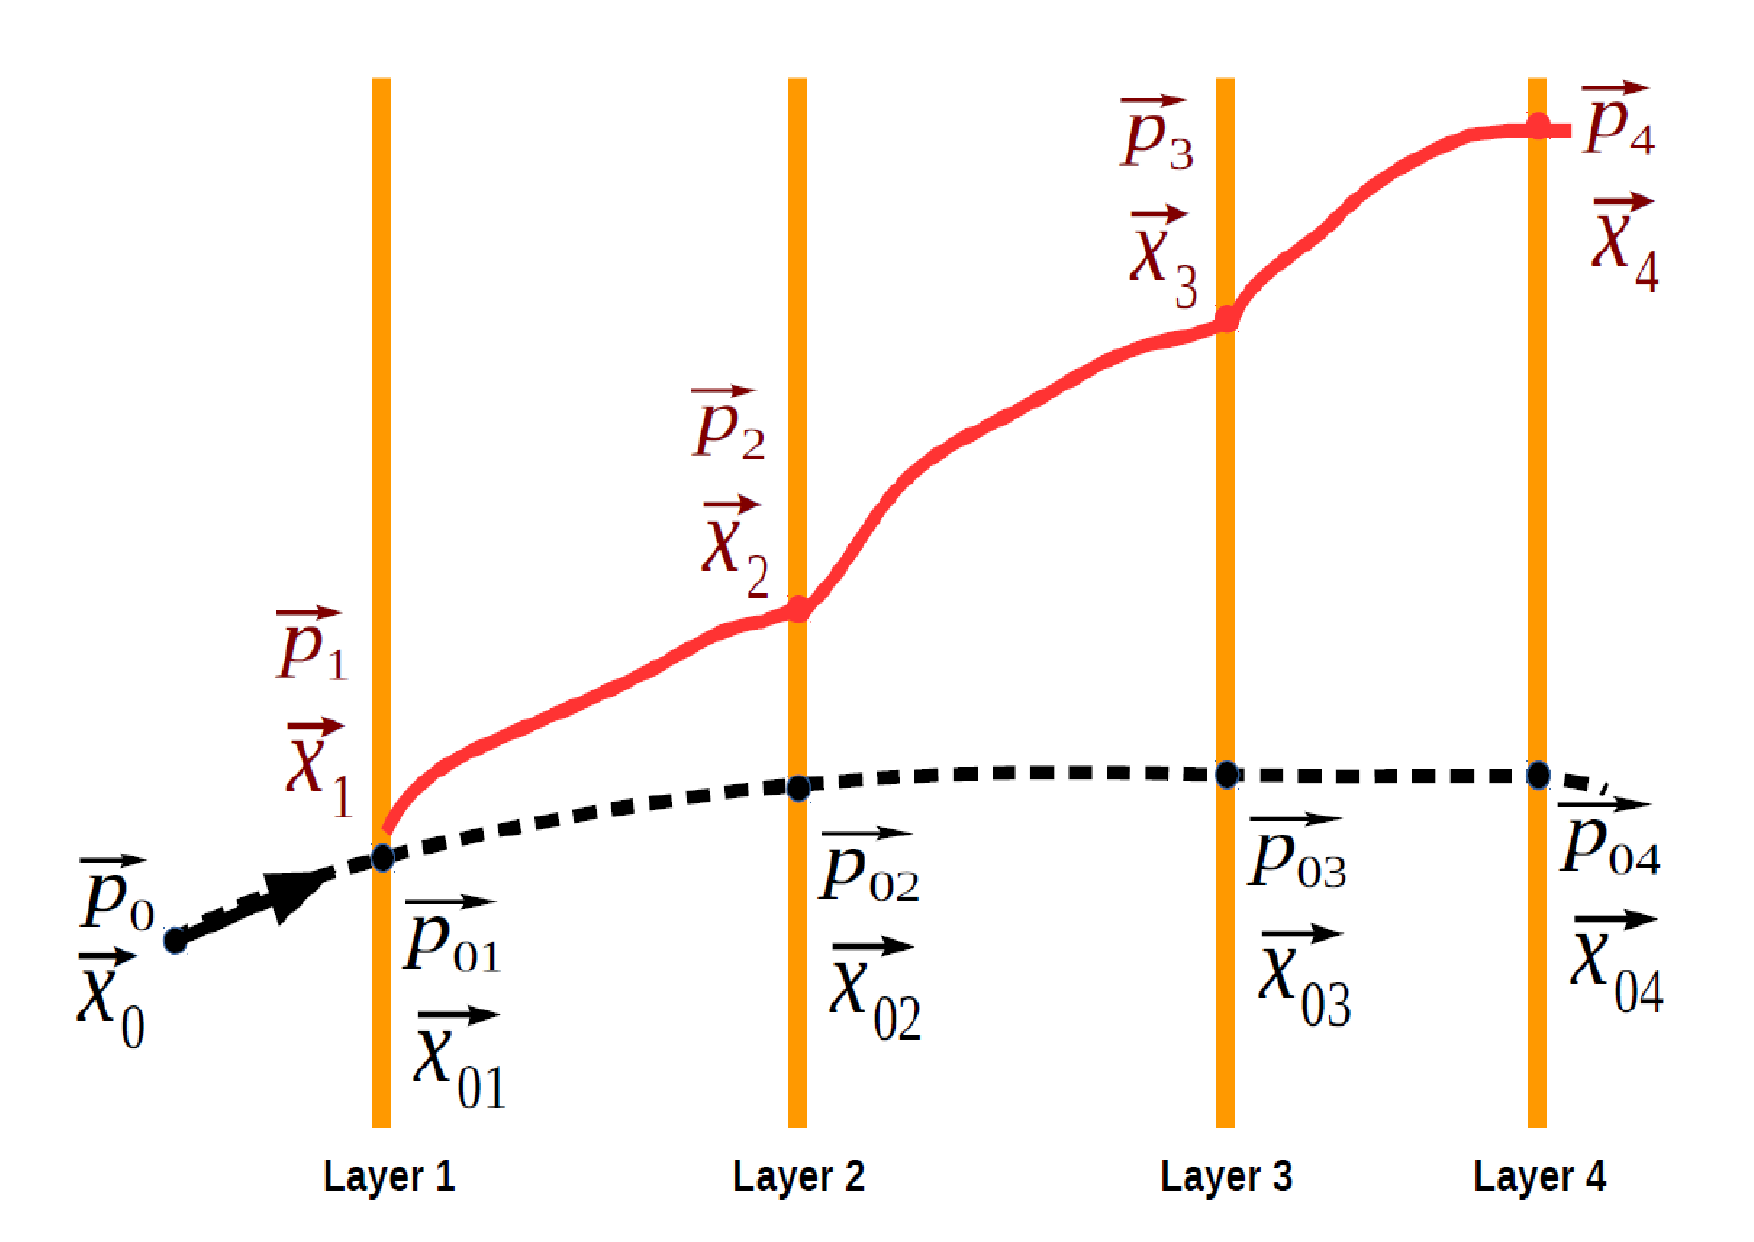
\includegraphics[width=0.7\textwidth]{figures/CalcSquem.pdf}
  \caption{Schematics for calculation of space point covariance matrix due to MS.}
  \label{fig:CalcSquem}
\end{figure}

The process begins with the calculation of the track average trajectory. This corresponds to trace the particle's trajectory 
ignoring MS and $E_{\rm loss}$ fluctuations, as these effects average out to zero. The trajectory will be the solution of the 
equation of motion within a magnetic field,

\begin{equation}
  \frac{d^2 \vec{r}}{ds^2} = \frac{q}{p}\frac{d\vec{r}}{ds}\times \vec{B},
\end{equation}
\noindent
where $q$ is the particles charge, $p$ is momentum magnitude which is constant, $\vec{B}$ the B-field and $s$ is the path-length along 
the trajectory. The solution of this equation for a given set of initial conditions, $\vec{x_0}$ and $\vec{p_0}$, can be written as,

\begin{equation}
  \vec{r} = \vec{f}(s;\vec{x}_0,\vec{p}_0).
\end{equation}
\noindent
The corresponding momentum along the trajectory is given by,
\begin{equation}
  \vec{p} = \vec{\kappa}(s;\vec{x}_0,\vec{p}_0) = p\frac{\partial \vec{f}(s;\vec{x}_0,\vec{p}_0)}{\partial s}.
\end{equation}

Lets suppose that the particle starts at the initial location $\vec{x_0}$ with momentum $\vec{p_0}$, and intersects a set of materials as 
shown in figure~\ref{fig:CalcSquem}. The black-dotted line shows the average trajectory. The red-solid line shows the actual trajectory
including the MS and $E_{\rm loss}$ fluctuations at the intersection with every material. The intersection coordinates and momenta, 
$\vec{x}_{0,i}$ and $\vec{p}_{0,i}$, of the average trajectory are given by

\begin{eqnarray}
  \vec{x}_{0,i} &=& \vec{f}(s_i;\vec{x_0},\vec{p_0})      = \vec{f}(s_i - s_{i-1};\vec{x}_{0,i-1},\vec{p}_{0,i-1}), \\
  \vec{p}_{0,i} &=& \vec{\kappa}(s_i;\vec{x_0},\vec{p_0}) = \vec{\kappa}(s_i - s_{i-1};\vec{x}_{0,i-1},\vec{p}_{0,i-1}).
\end{eqnarray}
\noindent

We start by considering the effects of MS. Lets denote the coordinates and momenta after intersecting the material of the actual particle trajectory by 
$\vec{x}_{i}$ and $\vec{p}_{i}$. At the intersection with layer-1 we have,

\begin{eqnarray}
  x^{k}_{1} &=& x^{k}_{0,1}, \\
  p^{k}_{1} &=& p^{k}_{0,1} + \delta p^{k}_{1};
\end{eqnarray}
\noindent
where $k=1,2,3$, and $\delta p^k_{1}$ is the effect of the multiple scattering at layer-1. This effect can be written as,

\begin{equation}
  \delta p^{k}_{1} = |\vec{p}_{01}|(\hat{m}^{k}_{11}\theta_{11} + \hat{m}^{k}_{12}\theta_{12}),
\end{equation}
\noindent
where $\hat{m}_{11}$ and $\hat{m}_{12}$ are any two mutually orthogonal unitary vector orthogonal to the momentum just 
previous to the intersection with the material; and $\theta_{11}$ and $\theta_{12}$ are the multiple scattering angles 
along the the $\hat{m}_{11}$ and $\hat{m}_{12}$ directions.

The coordinates and momenta of the actual trajectory just after layer-2 are given by,
\begin{eqnarray}
  \label{eq:x2}
  x^{k}_{2} &=& f^{k}(s_2 - s_1;\vec{x_1},\vec{p_1}) = f^{k}(s_2 - s_1;\vec{x}_{0,1},\vec{p}_{0,1} + \delta \vec{p}_{1}), \\
  p^{k}_{2} &=& \kappa^{k}(s_2 - s_1;\vec{x_1},\vec{p_1}) + \delta p^{k}_{2} = \kappa^{k}(s_2 - s_1;\vec{x}_{0,1},\vec{p}_{0,1} + \delta \vec{p}_{1}) + \delta p^{k}_{2};
\end{eqnarray}
\noindent
where
\begin{equation}
  \delta p^{k}_{2} = |\vec{p}_{02}|(\hat{m}^{k}_{21}\theta_{21} + \hat{m}^{k}_{22}\theta_{22}).
\end{equation}
\noindent
with $\hat{m}_{2i}$ and $\theta_{2i}$ a similar meaning as in the case of the intersection with layer-1.

\noindent
Equation~\ref{eq:x2} can be rewritten as,
\begin{eqnarray}
  x^{k}_{2} &=& f^{k}(s_2 - s_1;\vec{x}_{0,1},\vec{p}_{0,1})      + \frac{\partial f^{k}(s_2 - s_1;\vec{x}_{0,1},\vec{p}_{0,1})}{\partial p^{j}} \delta p^{j}_{1}      = x^{k}_{0,2} + \Delta x^{k}_{2}, \\
  p^{k}_{2} &=& \kappa^{k}(s_2 - s_1;\vec{x}_{0,1},\vec{p}_{0,1}) + \frac{\partial \kappa^{k}(s_2 - s_1;\vec{x}_{0,1},\vec{p}_{0,1})}{\partial p^{j}} \delta p^{j}_{1} + \delta p^{k}_{2} = p^{k}_{0,2} + \Delta p^{k}_{2};
\end{eqnarray}
\noindent
with
\begin{eqnarray}
  \label{eq:DelX2}
  \Delta x^{k}_{2} &=& {\mathcal F_{p}}^{kj}_{21} \delta p^{j}_{1}, \\
  \Delta p^{k}_{2} &=& {\mathcal K_{p}}^{kj}_{21} \delta p^{j}_{1}  + \delta p^{k}_{2};
\end{eqnarray}
\noindent
where the matrices ${\mathcal F_{p}}_{21}$ and ${\mathcal K_{p}}_{21}$ are given by
\begin{eqnarray}
  {\mathcal F_{p}}_{21} &=& \frac{\partial \vec{f}(s_2 - s_1;\vec{x}_{0,1},\vec{p}_{0,1})}{\partial \vec{p}}, \\
  {\mathcal K_{p}}_{21} &=& \frac{\partial \vec{\kappa}(s_2 - s_1;\vec{x}_{0,1},\vec{p}_{0,1})}{\partial \vec{p}}.
\end{eqnarray}

~\\
\noindent
In a similar fashion, the coordinates and momenta of the actual trajectory just after layer-3 are given by,
\begin{eqnarray}
  \label{eq:x3}
  x^{k}_{3} &=& f^{k}(s_3 - s_2;\vec{x_2},\vec{p_2}) = f^{k}(s_3 - s_2;\vec{x}_{0,2} + \Delta \vec{x}_{2},\vec{p}_{0,2} + \Delta \vec{p}_{2}), \\
  p^{k}_{3} &=& \kappa^{k}(s_3 - s_2;\vec{x_2},\vec{p_2}) + \delta p^{k}_{3} = \kappa^{k}(s_3 - s_2;\vec{x}_{0,1} + \Delta\vec{x}_{2},\vec{p}_{0,1} + \Delta \vec{p}_{2}) + \delta p^{k}_{3};
\end{eqnarray}
\noindent
with $\Delta \vec{x}_{2}$ and $\Delta \vec{p}_{2}$ given by Equation~\ref{eq:DelX2}, and $\delta p^{k}_{3}$ is the effect of MS after traversing the layer-3, with similar expression as in the 
previous cases. Again, Equation~\ref{eq:x3} can be rewritten as
\begin{eqnarray}
  x^{k}_{3} &=& x^{k}_{0,3}  + \frac{\partial f^{k}(s_3 - s_2;\vec{x}_{0,1},\vec{p}_{0,1})}{\partial x^{j}} \Delta x^{j}_{2} + \frac{\partial f^{k}(s_3 - s_2;\vec{x}_{0,1},\vec{p}_{0,1})}{\partial p^{j}} \Delta p^{j}_{2}, \\
  p^{k}_{3} &=& p^{k}_{0,2}  + \frac{\partial \kappa^{k}(s_3 - s_2;\vec{x}_{0,1},\vec{p}_{0,1})}{\partial x^{j}} \Delta x^{j}_{2} + \frac{\partial \kappa^{k}(s_3 - s_2;\vec{x}_{0,1},\vec{p}_{0,1})}{\partial p^{j}} \Delta p^{j}_{2} + \delta p^{k}_{2};
\end{eqnarray}
\noindent
which can be rewritten as
\begin{eqnarray}
  x^{k}_{3} &=& x^{k}_{0,3} + \Delta x^{k}_{2}, \\
  p^{k}_{3} &=& p^{k}_{0,3} + \Delta p^{k}_{2};
\end{eqnarray}
\noindent
with 
\begin{eqnarray}
  \label{eq:DelX3}
  \Delta x^{k}_{3} &=& {\mathcal F_{r}}^{kj}_{32} \Delta x^{j}_{2} + {\mathcal F_{p}}^{kj}_{32} \Delta p^{j}_{2}, \\
  \Delta p^{k}_{3} &=& {\mathcal K_{r}}^{kj}_{32} \Delta x^{j}_{2} + {\mathcal K_{p}}^{kj}_{32} \Delta p^{j}_{2}  + \delta p^{k}_{3};
\end{eqnarray}
\noindent
where the matrices ${\mathcal F_{r}}_{32}$, ${\mathcal F_{p}}_{32}$, ${\mathcal K_{r}}_{32}$ and ${\mathcal K_{p}}_{32}$ are given by
\begin{eqnarray}
  {\mathcal F_{r}}_{32} &=& \frac{\partial \vec{f}(s_3 - s_2;\vec{x}_{0,2},\vec{p}_{0,2})}{\partial \vec{x}}, \\
  {\mathcal F_{p}}_{32} &=& \frac{\partial \vec{f}(s_3 - s_2;\vec{x}_{0,2},\vec{p}_{0,2})}{\partial \vec{p}}, \\
  {\mathcal K_{r}}_{32} &=& \frac{\partial \vec{\kappa}(s_3 - s_2;\vec{x}_{0,2},\vec{p}_{0,2})}{\partial \vec{x}}, \\
  {\mathcal K_{p}}_{32} &=& \frac{\partial \vec{\kappa}(s_3 - s_2;\vec{x}_{0,2},\vec{p}_{0,2})}{\partial \vec{p}}.
\end{eqnarray}

~\\
\noindent
In general the $\Delta x^{k}_{n}$ and $\Delta p^{k}_{n}$ can be written as
\begin{eqnarray}
  \Delta x^{k}_{n} &=& \sum^{n-1}_{l = 1} F^{kj}_{n,l} \delta p^{j}_{l}, \\
  \Delta p^{k}_{n} &=& \sum^{n-1}_{l = 1} K^{kj}_{n,l} \delta p^{j}_{l} + \delta p^{j}_{n}.
\end{eqnarray}
\noindent
Where $\delta p^{j}_{l}$ is the MS effect just after layer-$l$ and given by,
\begin{equation}
  \delta p^{j}_{l} = |\vec{p}_{0l}|(\hat{m}^{j}_{1l}\theta_{1l} + \hat{m}^{j}_{1l}\theta_{1l}),
\end{equation}
\noindent
and where the $F^{kj}_{n,l}$ and $K^{kj}_{n,l}$ matrices are given by the recurrent formulas
\begin{equation}
  F^{kj}_{n,l} = \left\{
  \begin{array}{ll}
    {\mathcal F_{r}}^{km}_{n,n-1} F^{mj}_{n-1,l} + {\mathcal F_{p}}^{km}_{n,n-1} K^{mj}_{n-1,l} & \mbox{if } l < n-1 \\
    {\mathcal F_{p}}^{km}_{n,n-1}                                                               & \mbox{if } l = n-1
   \end{array}
  \right.
\end{equation}
\noindent
and 
\begin{equation}
  K^{kj}_{n,l} = \left\{
  \begin{array}{ll}
    {\mathcal K_{r}}^{km}_{n,n-1} F^{mj}_{n-1,l} + {\mathcal K_{p}}^{km}_{n,n-1} K^{mj}_{n-1,l} & \mbox{if } l < n-1 \\
    {\mathcal K_{p}}^{km}_{n,n-1}                                                               & \mbox{if } l = n-1
   \end{array}
  \right.
\end{equation}

\noindent
This allows to calculate the covariance matrix due to MS among the $\Delta x^{k}_{n}$ as follows
\begin{equation}
  \label{eq:Cov_X_MS_1}
  \left<  \Delta x^i_n x^j_m \right >_{\rm MS} = \sum^{n-1}_{l=1}\sum^{m-1}_{a=1} F^{ik}_{n,l} F^{jb}_{m,a} \left< \delta p^{k}_{l} \delta p^{b}_{a} \right>.
\end{equation}
\noindent
The covariance matrix among the $\delta p^k_l$ is given by
\begin{equation}
  \left< \delta p^{k}_{l} \delta p^{b}_{a} \right> = |\vec{p}_{0l}||\vec{p}_{0a}| (\hat{m}^k_{1l}\hat{m}^b_{1a} \left< \theta_{1l}\theta_{1a} \right> + \hat{m}^k_{1l}\hat{m}^b_{2a} \left< \theta_{1l}\theta_{2a} \right> + \hat{m}^k_{2l}\hat{m}^b_{1a} \left< \theta_{2l}\theta_{1a} \right> + \hat{m}^k_{2l}\hat{m}^b_{2a} \left< \theta_{2l}\theta_{2a} \right> )
\end{equation}
\noindent
The MS angles $\theta_{ik}$ are totally uncorrelated, {\it i.e.} $\left< \theta_{kl}\theta_{ma} \right> = \delta_{km}\delta_{la}(\theta^0_{l})^2$, with $\theta^0_{l}$ the mean-root-square 
of the MS angle at layer-$l$, which is given by the usual formula~\cite{bib:MS_angle},
\begin{equation}
  \theta^{0}_{l} = \frac{13.6~{\rm MeV/c}}{c\beta_{0,l}p_{0,l}} q \sqrt{x/X_0} \left[ 1 + 0.038 ln(x/X_0) \right],
\end{equation}
\noindent
where $q$, $p_{0,l}$, $c\beta_{0,l}$, are the charge number, momentum and velocity of the incident particle, and $x/X_0$ is the thickness of the scattering medium in radiation lengths.

Finally, $\left<  \Delta x^i_n x^j_m \right >_{\rm MS}$ can be written as follows,
\begin{equation}
  \left<  \Delta x^i_n x^j_m \right >_{\rm MS} = p^2 \sum^{n-1}_{l=1}\sum^{m-1}_{a=1} F^{ik}_{n,l} F^{jb}_{m,a} \left(\hat{m}^k_{1l}\hat{m}^b_{1a} + \hat{m}^k_{2l}\hat{m}^b_{2a}\right) \delta_{la} (\theta^0_l)^2,
\end{equation}
\noindent
where $p$ is the particle's momentum.


~\\
\noindent
A similar calculation can be used for the energy loss fluctuations. It is only needed to replace in eq.~\ref{eq:Cov_X_MS_1} the corresponding expression for the $\left< \delta p^{k}_{l} \delta p^{b}_{a} \right>$.
The $\delta p^{k}_{l}$ due to energy loss fluctuations can be written as,

\begin{equation}
  \delta p^{k}_{l} = \left(\frac{E}{p}\right) \hat{p}^{k}_{l} \sigma^{l}(E_{\rm loss}),
\end{equation}
\noindent
where $E/p$ is the particle's energy-momentum ratio, $\hat{p}^{k}_{l}$ is the $k$-component of the particle's momentum direction at intersection $l$, and 
$\sigma^{l}(E_{\rm loss})$ is the $E_{\rm loss}$ RMS at intersection $l$. For this last one we use a simple model proposed by the ALICE collaboration, 

\begin{equation}
  \label{eq:sigmaEloss}
  \sigma^{l}(E_{\rm loss}) = \kappa \times \sqrt{E^l_{\rm loss}},
\end{equation}
\noindent
where ${E^l_{\rm loss}}$ is calculated from the famous $dE/dx$ Bethe-Bloch formula~\cite{bib:MS_angle}, and $\kappa$ is a parameter which has been tuned to the value 0.015 
when the both $\sigma^{l}(E_{\rm loss})$ and $E^l_{\rm loss}$ are expressed in ${\rm GeV}$. The $\kappa$-tunning has being made by comparing the {\guari} output with the ILD 
full-simulation tracking performances. We can now calculate $\left< \delta p^{k}_{l} \delta p^{b}_{a} \right>$ due to the $E_{\rm loss}$ fluctuation,

\begin{equation}
  \left< \delta p^{k}_{l} \delta p^{b}_{a} \right> = \left( \frac{E}{p} \right)^2 \left(\hat{p}^{k}_{l}\hat{p}^{b}_{a}\right)\delta_{la}\sigma^{l}(E_{\rm loss}),
\end{equation}
\noindent
where the $\delta_{la}$ is due to the independence of the $E_{\rm loss}$ fluctuations at the different intersections.

Finally, $\left<  \Delta x^i_n x^j_m \right >_{E_{\rm loss}}$ can be written as follows,
\begin{equation}
  \left<  \Delta x^i_n x^j_m \right >_{E_{\rm loss}} = \left( \frac{E}{p} \right)^2 \sum^{n-1}_{l=1}\sum^{m-1}_{a=1} F^{ik}_{n,l} F^{jb}_{m,a} \left(\hat{p}^k_l\hat{p}^b_{a}\right) \delta_{la} \sigma^{l}(E_{\rm loss}).
\end{equation}


~\\
\noindent
In {\guari} package the measurement coordinates are expressed in terms of the sensor's local reference frame $\vec{x'}$, where the third coordinate is always perpendicular to the sensitive surface. 
The latest are functions of the global coordinates $\vec{x}$. The covariance matrix among the measurement coordinates in the sensor's local frame can be written as,

\begin{eqnarray}
  \left<  \Delta x'^i_n x'^j_m \right > &=& \delta_{ij}\delta_{nm}\sigma^i_n\sigma^j_m + \frac{\partial x'^i_n}{\partial x^k_n} \frac{\partial x'^j_m}{\partial x^r_m} \left( \left<  \Delta x^k_n x^r_m \right >_{\rm MS} + \left<  \Delta x^k_n x^r_m \right >_{E_{\rm loss}} \right) \\
                                        &=& V_{\rm sp} + V_{MS} + V_{E_{\rm loss}},
\end{eqnarray}
\noindent
where the first term describes the sensor's intrinsic resolution, the second the MS and the third the $E_{\rm loss}$ fluctuations.

~\\
Finally, the expression for the track parameters covariance matrix can be calculated as follows. Lets arrange the set of measurement coordinates in the array $\Gamma^{\rm meas}_i$, and lets 
$\Gamma_i(\vec{\alpha})$ be the track intersection coordinates with the different measurement layers as a function of the track parameters $\vec{\alpha}$. As an example, in the case of a straight 
line (helix) $\vec{\alpha}$ is a vector of size 4 (5). The track fitting consist at minimizing the $\chi^2$ given by

\begin{equation}
  \chi^2 = \sum_{i,j} (\Gamma_i(\vec{\alpha}) - \Gamma^{\rm meas}_i) \left(V\right)^{-1}_{ij} (\Gamma_j(\vec{\alpha}) - \Gamma^{\rm meas}_j),
\end{equation}
\noindent
where $V$ is the total covariance matrix $V = V_{\rm sp} + V_{MS} + V_{E_{\rm loss}}$. The track parameters covariance matrix is given by
\begin{equation}
 \left(V_{\vec{\alpha}} \right)^{-1}_{km} = \frac{1}{2}\frac{\partial^2\chi^2}{\partial \alpha_k \partial \alpha_m} = \sum_{i,j} \frac{\partial \Gamma_i(\vec{\alpha})}{\partial \alpha_k} \left(V \right)^{-1}_{ij} \frac{\partial \Gamma_j(\vec{\alpha})}{\partial \alpha_m}.
\end{equation}
\noindent
where the derivatives are evaluated at the actual known values of the track parameters, which can be easily calculated from the initial conditions $\vec{x}_0$ and $\vec{p}_0$ at the particle's origin.

\subsection{Tracking efficiency calculation}
\label{subsec:TrkEffic_calculation}

The tracking efficiency calculation depends on the track-finding algorithm used. For the time being only one such algorithm has been implemented and described in the next section.
Later in this document (c.f. sec.~\ref{subsec:track_finder_class}) some guide lines to implement a new pattern recognition algorithms will be given.

\subsubsection{FPCCD track finder}
\label{subsubsec:FPCCDTrkEffic_calculation}

This track finder is inspired in the FPCCD track-finder, one of the pattern recognition algorithms used by the ILD collaboration~\cite{bib:ILD_FPCCD_TrackFinder}, which
was developed to take advantage of fine pixel CCD silicon sensors. The tracking efficiency calculation that will be detailed here below uses the same features as the ALICE 
ITS Upgrade fast-simulation~\cite{bib:ALICE_fastsim}.

The procedure starts by calculating the efficiency ($P_{\rm seed}$) of so-called seeding configurations, which consist of sets of three layers for the reconstruction of a seed 
track. The set of seed configurations should be adapted to the application and has to be defined by the user. The seed track parameters covariance matrix is then calculated and 
used to obtain the track pointing resolution at the next sensitive layer. If previous to that an insensitive layer is intersected, the track parameters covariance matrix is updated 
including the MS and $E_{\rm loss}$ fluctuations of the insensitive layer. This track pointing resolution is then used to calculate the probability of good, fake or null track-hit 
association ($P_l$). If a hit is associated (either good or fake) the track parameters covariance matrix is updated adding this new measurement point. The extrapolation process is 
continued until no more sensitive layers are found.

The tracking efficiency of a given seed configuration with the corresponding configuration of associated good, fake and null hits is given by,

\begin{equation}
 \epsilon^k = P^k_{\rm seed} \prod_l P_l,
\end{equation}
\noindent
where $P^k_{\rm seed}$ is the efficiency for the seeding configuration $k$ and $P_l$ is the probability of either good, fake or null track-hit association at layer $l$. This equation 
ignores possible correlations among the seeding efficiency and the track-hit associations of the subsequent layers.

The total tracking efficiency is given by
\begin{equation}
 \epsilon = \sum_k \epsilon^k,
\end{equation}
\noindent
where the sum runs over all the seeding configurations plus associated hits respecting some constrains such as: minimum number of hits in the track, minimum purity 
(\# good hit association)/(\# total hits), ...

Each configuration $k$ will have as well its own track parameters covariance matrix $V^k_{\vec{\alpha}}$. The average covariance matrix will be give by,

\begin{equation}
 \left< V_{\vec{\alpha}} \right>  = \frac{\sum_k \epsilon^k V^k_{\vec{\alpha}} } { \sum_k \epsilon^k }.
\end{equation}
\noindent
The output of the whole calculation will then be the tracking efficiency as well as the average track parameters covariance matrix.

~\\
\noindent
In the following sub-sections are detailed the calculations for the seeding configuration efficiency and the track-hit association probabilities.

\subsubsection*{Seeding probability calculation}

As mentioned above, the seeding configurations are a list of combinations of three layers used to reconstruct a seed track. The actual combinations are application 
dependent and should then be specified by the user. In the process of pattern recognition in a real experiment the list of seed configurations will be hierarchized, 
starting by the most likely one. In a collider experiment with a tracker with cylindrical symmetry with respect to the beam lines the seeding should start with 
combinations of the outermost layers, the ones with the lower hit rates density (hit per unit of time per unit of surface), as this reduces the amount of combinatorics.
If some of the track hits on the outermost layers go undetected the corresponding seeding configuration will not be found. In order to increase tracking efficiency 
some other combinations with inner layers could also be tested but at the expense of increased combinatorics.

The seeding efficiency is modeled as the product of three components,

\begin{equation}
 P_{\rm seed} = P({\rm intrinsic}) P(p^{\rm min}_t) P(\chi^2/ndf~cut),
\end{equation}
\noindent
where $P({\rm intrinsic})$ is the intrinsic probability of the seeding configuration, $P(p^{\rm min}_t)$ the probability for the seed configuration to pass a 
minimum $p^{\rm min}_t$ cut, and $P(\chi^2/ndf~cut)$ the probability of the seed track to pass a maximum $\chi^2/ndf$ cut.

$P(\chi^2/ndf~cut)$ is easily calculated as the probability for a $\chi^2$ distribution with $ndf$ degrees of freedom to be smaller than a certain maximum $(\chi^2/ndf)_{\rm max}$ 
specified by the user. The $ndf$ is calculated as the difference $ndf = 2n_{\rm hits} - n_{\rm trk-params}$, where $n_{\rm hits}$ is the number of hits to reconstruct 
the seed track (in this case three) and $n_{\rm trk-params}$ is the number of track parameters (in this case five).

$P({\rm intrinsic})$ depends on the number of good, fake and null hits related with the seed configuration. This will be easier to understand by considering an example. 
Lets consider a track that intersects the four outermost layers of a tracker, denoted by $l_1$, $l_2$, $l_3$, $l_4$, respectively. The following set of seed configurations 
could be specified,

\begin{itemize}
 \item  $(l_2,l_3,l_4)$,
 \item  $(l_1,l_3,l_4)$,
 \item  $(l_1,l_2,l_4)$,
 \item  $(l_1,l_2,l_3)$.
\end{itemize}
\noindent
The first configuration $(l_2,l_3,l_4)$ corresponds to a seed track with hits on the 3 outermost layers. The intrinsic probability for this configuration is given by 
$P^2_{\rm hit} P^3_{\rm hit} P^4_{\rm hit}$, where $P^k_{\rm hit}$ is the probability of having either a good or fake hit at layer $k$. The second
configuration $(l_1,l_3,l_4)$ means that no hit was found at layer $2$, so the intrinsic probability is given by $P^1_{\rm hit} P^2_{\rm null} P^3_{\rm hit} P^4_{\rm hit}$, 
where $P^2_{\rm null}$ is the probability of not finding a hit on layer 2. The other seed configurations will have similar expressions.

The probability for finding a good hit in the seed layer $k$ ($P^k_{\rm good}$) is simply the layer intrinsic detection efficiency $P^k_{\rm good} = \epsilon^k_{\rm det}$. 
The probability for no hit in the seed layer $k$ ($P^k_{\rm null}$) is given by the product of not detecting the real track hit ($1 - \epsilon^k_{\rm det}$) and 
not finding a fake hit ($P^k_{\rm no-fake}$),

\begin{equation}
 P^k_{\rm null} = (1 - \epsilon^k_{\rm det}) P^k_{\rm no-fake}.
\end{equation}
\noindent
$P^k_{\rm no-fake}$ is calculated by using the layer hit rate $R^k_{\rm bkg}$, read-out time $t^k_{\rm r.o.}$ and a surface $S^k$. The average number of fake hit 
will be given by $N^k_{\rm bkg} = R^k_{\rm bkg} t^k_{\rm r.o.} S^k$. Assuming that the number of fake hits are Poisson distributed, $P^k_{\rm no-fake}$ is 
given by,

\begin{equation}
  P^k_{\rm no-fake} = Poisson(0,N^k_{\rm bkg}) = e^{-N^k_{\rm bkg}}.
\end{equation}
\noindent
The last element to define is the surface $S^k$. This is given by the size of the region where the real track hits have a sizable probability. This is given by the 
surface of the $1-\sigma$ ellipse ($S^k_{1\sigma}$), which includes the sensor intrinsic resolution, MS and $E_{\rm loss}$ fluctuations, multiplied the a factor related 
to the $(\chi^2/ndf)_{\rm max}$ on the seed track,

\begin{equation}
  S^k = \left[(\chi^2/ndf)_{\rm max}\right]^{1/2} S^k_{1\sigma}.
\end{equation}
\noindent
The probability of finding a fake hit at the seed layer $k$ ($P^k_{\rm fake}$) is given by,

\begin{equation}
  P^k_{\rm fake} = 1 - P^k_{\rm good} - P^k_{\rm null} = (1 - \epsilon^k_{\rm det}) (1 - P^k_{\rm no-fake}).
\end{equation}

~\\
\noindent
The Last component of the seeding efficiency to discuss is the term related to the $p^{\rm min}_t$ cut, $P(p^{\rm min}_t)$. This term is characteristic of the FPCCD pattern 
recognition algorithm, which track seeding process is illustrated in figure~\ref{fig:FPCCD_Seeding}. This algorithm looks for a hit in the outermost seed layer of a given 
seeding configuration. If a hit is found then it proceeds to draw on the plane perpendicular to the uniform magnetic field two hypothetical tracks generated at the center-point, 
going through the hit on the outer layer, having $p_t = p^{\rm min}_t$ and having a $\pm1$ electric charge. This defines a search window for looking for hits in the other inner seed 
layers. If hits are found within this search window, then the track is fit and a $(\chi^2/ndf)_{\rm max}$ cut is applied. This is how a $p^{\rm min}_t$ cut is applied on the seed 
tracks. The efficiency due to this $p^{\rm min}_t$ cut should be 0 (1) for tracks with $p_t$ much below (above) $p^{\rm min}_t$, and should show a quick $0 \rightarrow 1$ transition 
for $p_t$ around $p^{\rm min}_t$.

\begin{figure}
  \centering
  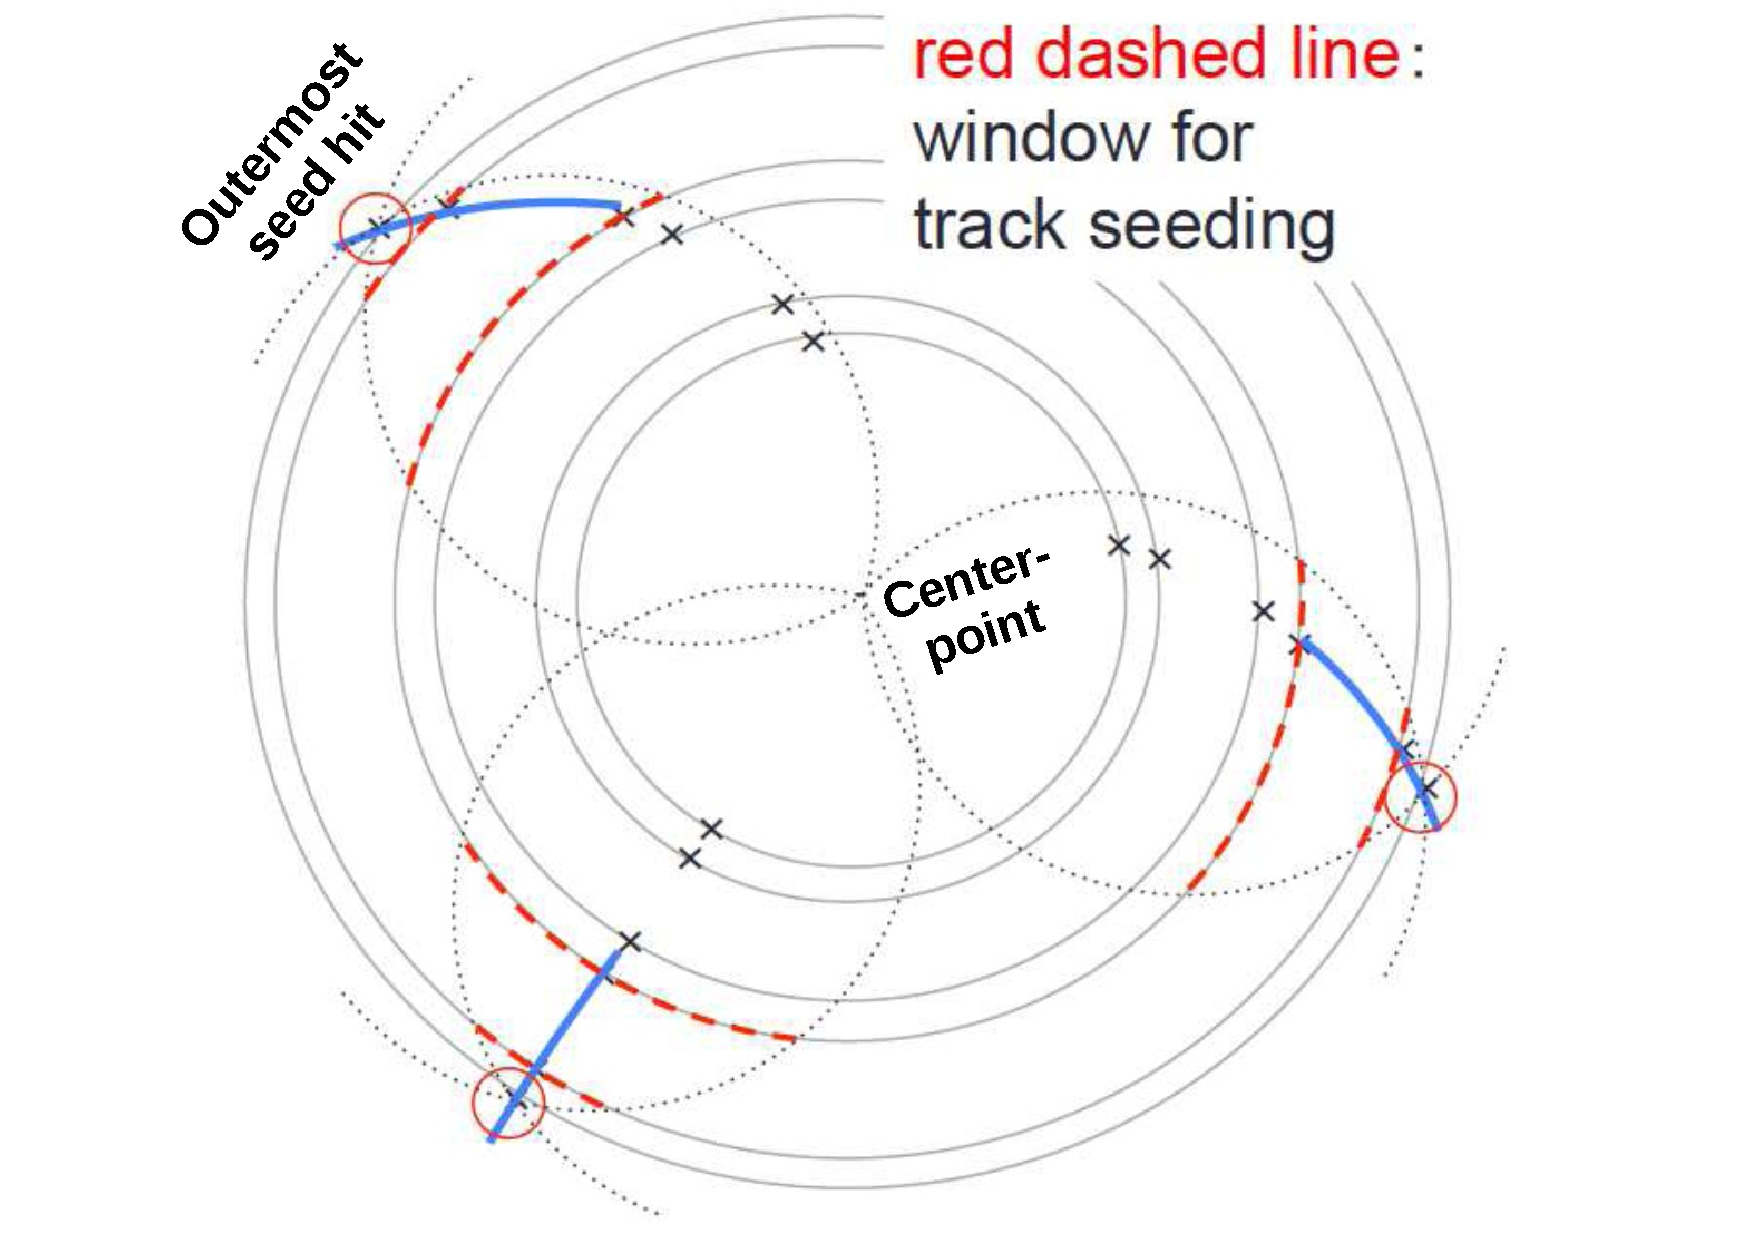
\includegraphics[width=0.6\textwidth]{figures/FPCCD_Seeding.pdf}
  \caption{Graphical representation of track seeding process for the FPCCD track-finder algorithm. Crosses denote hits on the tracker. 
  Crosses surrounded by red circles in the outer layer are used to determine a wide enough search region to catch track seeds with $p_t > p^{\rm min}_t$. 
  Dotted curved lines denote tracks passing through the outermost seed hit, through a center-point and with $p_t = p^{\rm min}_t$. Red dashed lines 
  denote search windows for generating track seeds, and their length is determined by intersections between layers and the dotted curved lines. Blue 
  curved lines denote the track seeds generated by this process.}
  \label{fig:FPCCD_Seeding}
\end{figure}

In this package this $p^{\rm min}_t$ cut seed efficiency is calculated with a MC method. For this the three seed hits are sampled $N_{\rm sampling}$ times with a multi-variate 
Gaussian distribution with the their actual covariance matrix. For each sampling, the outermost seed hit is used to define the search window as described above. It is then 
count the amount of samplings ($N_{\rm passed}$) in which the two innermost seed hits were found inside such search window. The efficiency is then simply defined as,

\begin{equation}
 P(p^{\rm min}_t) = \frac{N_{\rm passed}}{N_{\rm sampling}}.
\end{equation}
\noindent
For this calculation $N_{\rm sampling}$ should be defined by the user by finding a trade-off between precision and calculation time.

\subsubsection*{Track-hit association probabilities}

The track-hit association probability at a layer $l$ depends on the track pointing resolution onto the layer, the layer intrinsic resolution and the hit rate at this layer. 
The hit rate depends on many factors and tries to include effects such as sensor electric noise, event multiplicity, background and possible pile-up.

One can show that the probability that the correct cluster will be associated to extrapolated seed with smaller $\chi^2$ than any random hits can be expressed as 
(assuming infinite size search-window),

\begin{equation}
 P^{l}_{\rm corr} = \frac{\epsilon^l_{\rm det}}{1 + N^l_{\rm bkg}},
\end{equation}
\noindent
where $\epsilon^l_{\rm det}$ is the layer intrinsic detection efficiency and $N^l_{\rm bkg}$ is the expected number of fake hits within the region $S^l$ defined 
by the convolution of the track pointing resolution and the layer intrinsic resolution, {\it i.e.} $N^l_{\rm bkg} = R^l_{\rm bkg} t^l_{\rm r.o.} S^l$.
The above can be extended to use search windows of finite size. The correct track-hit association probability is then transformed to,

\begin{equation}
  P^{l}_{\rm corr} = \frac{\epsilon^{l}_{\rm det} \left( 1 - \gamma^{1 + N^l_{\rm bkg}} \right)}{1 + N^l_{\rm bkg}},
\end{equation}
\noindent
where $\gamma$ is the fraction of correct hits lost to the $\chi^2$ cut in the track-hit association process ({\it e.g.} $\gamma \simeq 5\%$ with $\chi^2/ndf < 3$ cut). 
The probability of no track-hit association is then,

\begin{equation}
  P^{l}_{\rm null} = \left(1 - \epsilon^l_{\rm det} + \epsilon^l_{\rm det}\gamma \right)  \gamma^{N^l_{\rm bkg}},
\end{equation}
\noindent
and finally, the probability to have a fake associated to the track is,
\begin{equation}
  P^{l}_{\rm fake} = 1 - P^l_{\rm corr} - P^l_{\rm null}.
\end{equation}


Therefore, three states (correct, fake and no association) are possible per layer. The number of possible outcomes also depends on the number of layers and is therefore $K_p =3^N$. 
Only one outcome corresponds to the simplified picture of correct cluster association on each single layer ($N$ correct track-hit associations). By adding the probabilities of {\it e.g.} 
having $N - 1$ correct associations and no association at the remaining layer would correspond to "correct tracks with at least $N - 1$ clusters" and so on.


